En esta sección se hará un panorama general de los paneles de usuario implementados en el juego principal, 
que permiten a los jugadores gestionar su experiencia de juego, personalizar su personaje, 
revisar su progreso y acceder a diversas funcionalidades dentro del juego.

\subsubsection{Interfaz del menú principal}

El menú principal del juego es la primera pantalla que los jugadores ven al iniciar el juego. 
Desde aquí, los jugadores, una vez hayan iniciado sesión, pueden acceder al navegador principal de mundos, 
donde pueden explorar y unirse a diferentes mundos creados por otros jugadores creadores.

\begin{figure}[H]
    \centering
    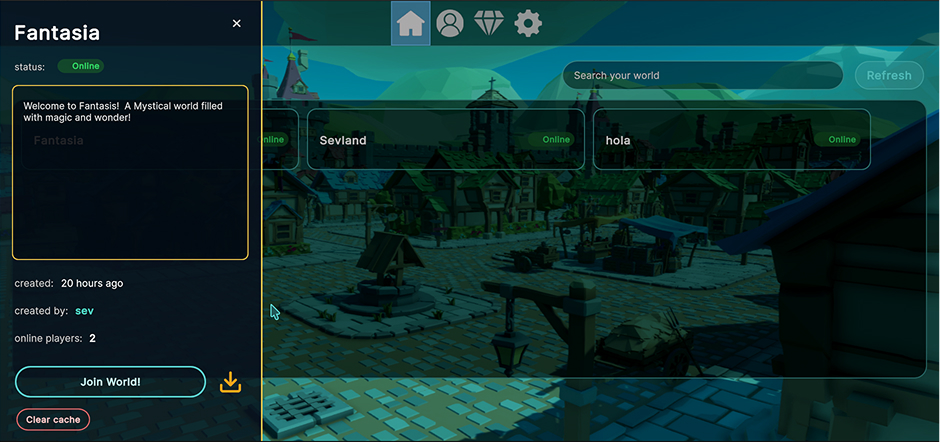
\includegraphics[width=1\textwidth]{img/08-implemented-solution/product/world-feed.jpg}
    \caption{Captura de pantalla del navegador de mundos.}    \label{fig:world-feed}
\end{figure}

Dentro del mismo menú principal, los jugadores también pueden acceder a su perfil de usuario, donde pueden 
modificar su nombre que se muestra dentro del juego, y cambiar su avatar también mostrado dentro del juego, 
eligiendo entre una variedad de opciones de personalización disponibles de cada parte de su personaje, 
como el peinado, la ropa, los accesorios, etc. Además, como se menciona en otras secciones, aquí se muestran 
los cosméticos que el jugador ha adquirido, y que puede equipar para personalizar aún más su apariencia dentro 
del juego, que haya coleccionado de distintos mundos y este se puede visualizar y ser visualizado por otros jugadores.

\begin{figure}[H]
    \centering
    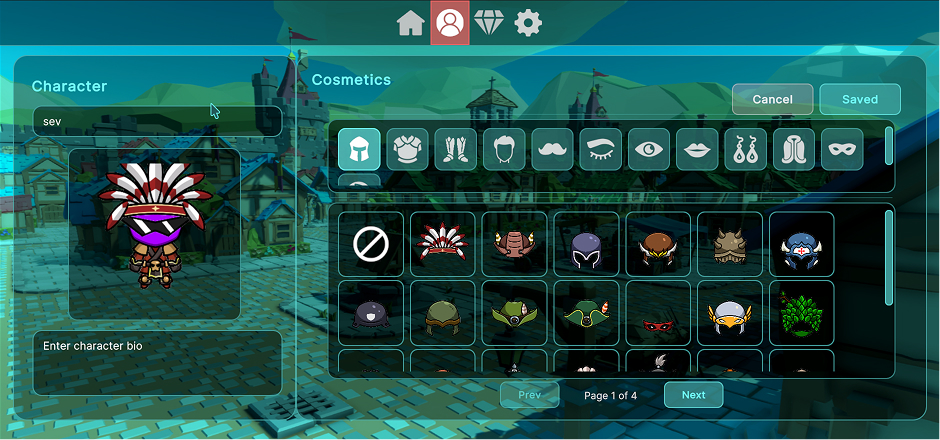
\includegraphics[width=1\textwidth]{img/08-implemented-solution/product/character-edit.jpg}
    \caption{Captura de pantalla del editor de personajes.}    \label{fig:character-edit}
\end{figure}


Otra sección dentro del menú, es la sección de adquisición de gemas, donde los jugadores pueden comprar gemas 
con dinero real a través de la plataforma de pago integrada, y una vez hecha la adquisición, las gemas se 
añaden a su cuenta de usuario y pueden ser utilizadas para comprar cosméticos y otros artículos dentro del juego
en el shop de cada mundo.


\begin{figure}[H]
    \centering
    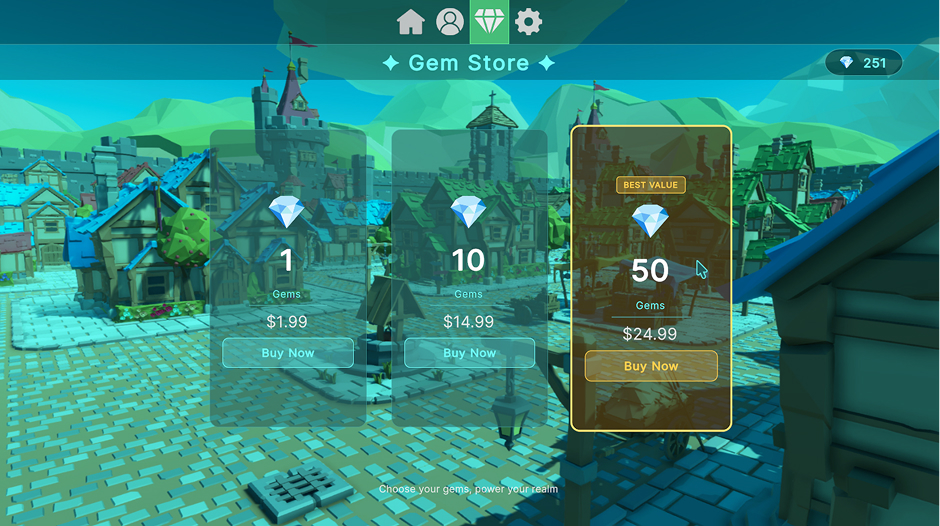
\includegraphics[width=1\textwidth]{img/08-implemented-solution/product/gem-store.jpg}
    \caption{Captura de pantalla de la tienda de gemas.}    \label{fig:gem-store}
\end{figure}


Por último, otra sección es la de configuración, donde los jugadores pueden ajustar el sonido, la música, 
la resolución gráfica y eliminar el cache que utiliza el juego. El juego presenta música y efectos de sonido 
integrados en el menú principal, y durante la sesión del juego. Un menú de configuración similar también está 
disponible dentro del juego, por lo que puede modificarse de ambos lugares y persiste su configuración al cambiar 
entre el menú principal y el juego, y al momento de iniciar el juego se cargan los últimos ajustes hechos. 

\begin{figure}[H]
    \centering
    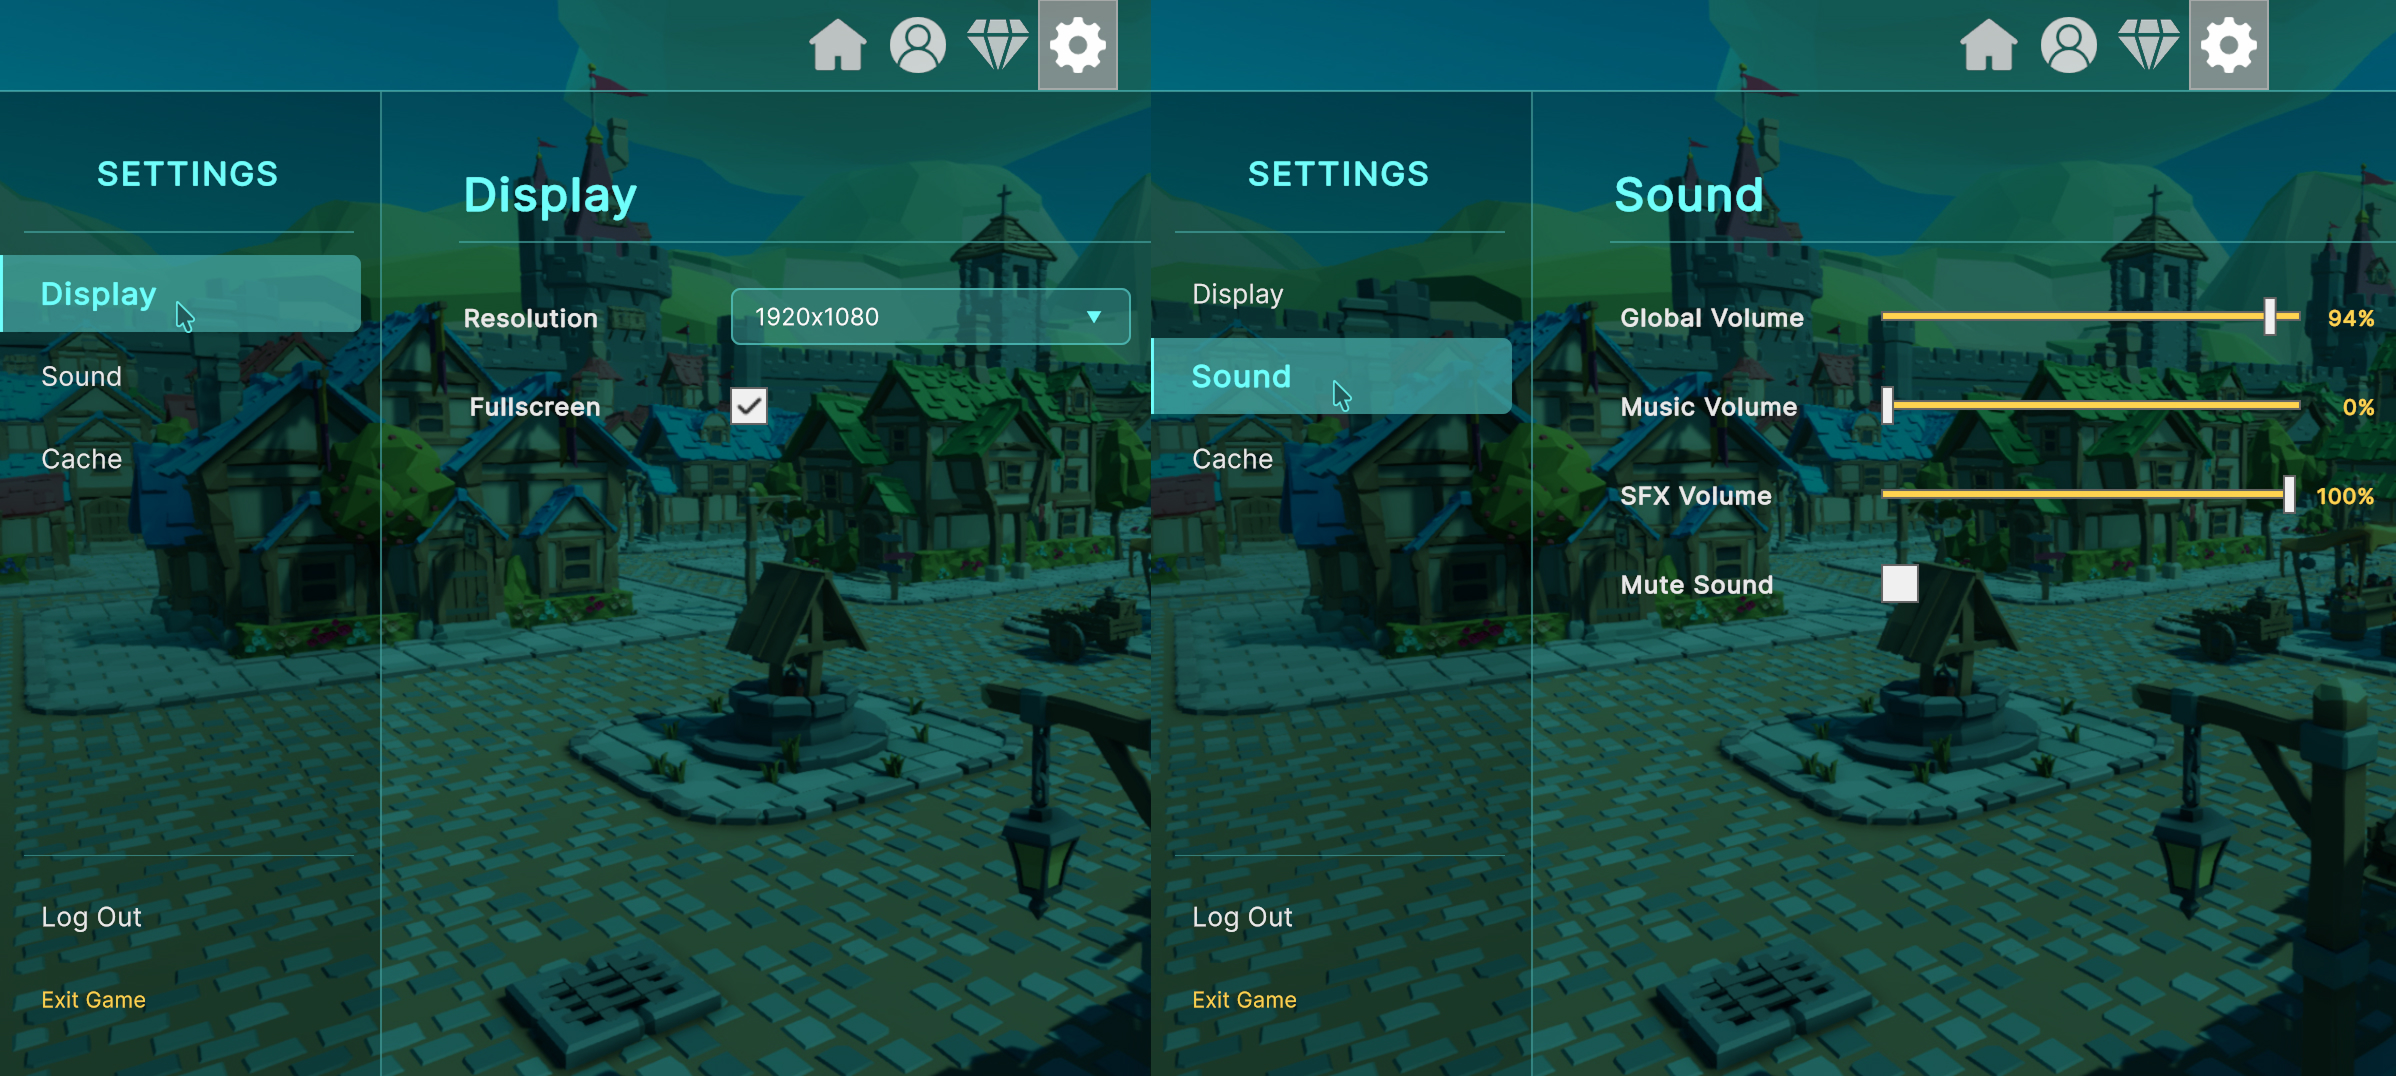
\includegraphics[width=0.55\textwidth]{img/08-implemented-solution/product/settings.jpg}
    \caption{Captura de pantalla de la configuración.}    \label{fig:settings}
\end{figure}

\subsubsection{Interfaz del juego}

Una vez dentro del juego, los jugadores tienen acceso a un \textit{HUD} (Heads-Up Display o Visualizacion 
de Interfaz en la Pantalla) que les proporciona información esencial sobre su personaje, su entorno y sus interacciones. 
El \textit{HUD} incluye elementos como la barra de salud, la barra de energía, sus monedas actuales, el 
inventario de acceso rápido y el seguimiento de misiones. 

\begin{figure}[H]
    \centering
    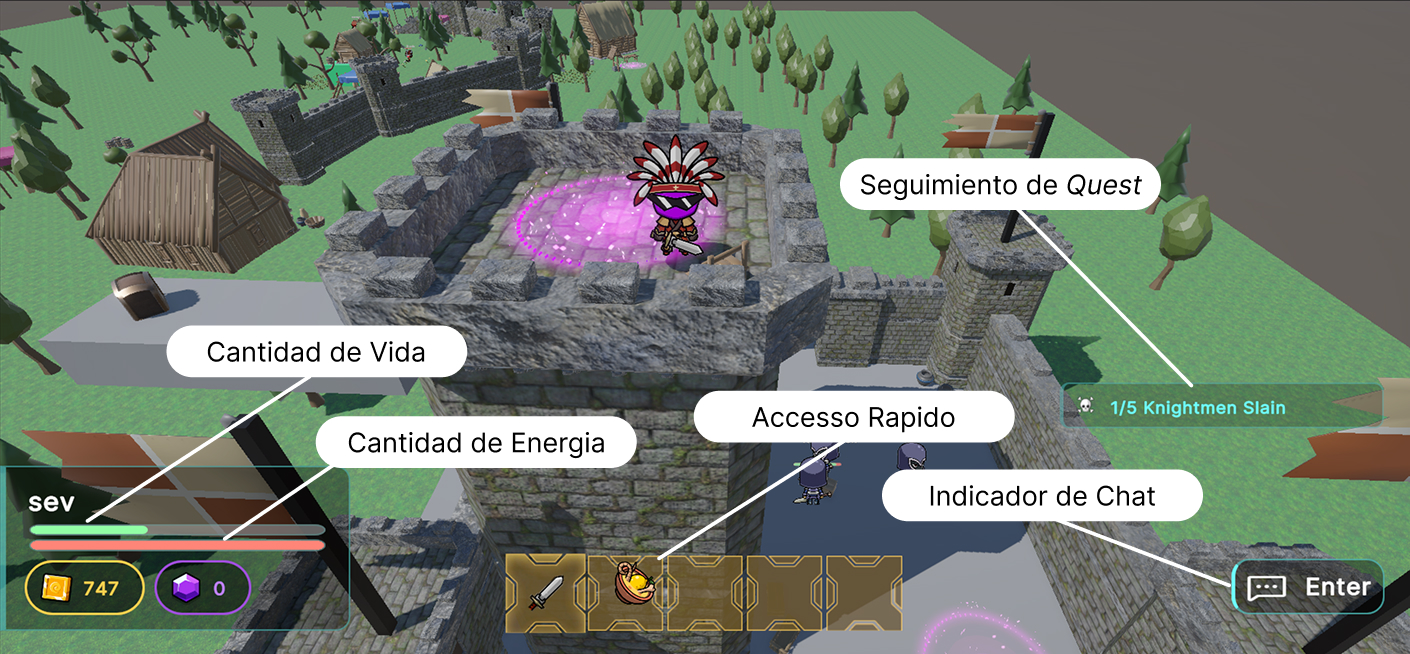
\includegraphics[width=0.85\textwidth]{img/08-implemented-solution/product/hud.jpg}
    \caption{Captura de pantalla del HUD.}    \label{fig:hud}
\end{figure}


Además del \textit{HUD}, los jugadores pueden acceder a un menú inventario completo, donde pueden organizar su inventario, 
equipar armas y consumibles, y revisar las estadísticas de los items.


\begin{figure}[H]
    \centering
    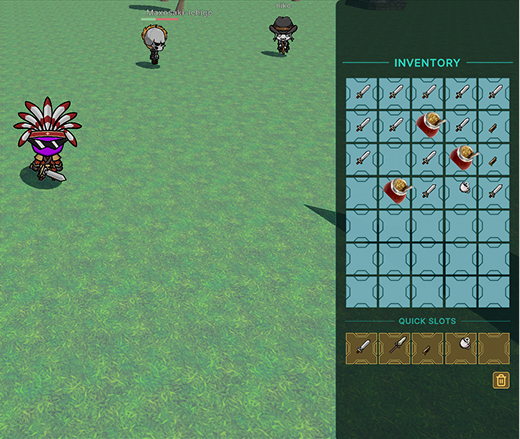
\includegraphics[width=0.65\textwidth]{img/08-implemented-solution/product/inventory.jpg}
    \caption{Captura de pantalla del inventario.}    \label{fig:inventory}
\end{figure}


Con respecto a las misiones, los jugadores pueden acceder a un menú de misiones donde pueden revisar las misiones 
activas, sus objetivos y su progreso. Este menú también proporciona información sobre las misiones completadas, 
permitiendo a los jugadores mantenerse organizados. Dentro de este menú se puede modificar la lista del seguimiento 
de misiones, para mostrar solo las misiones que el jugador desea seguir en su HUD.


\begin{figure}[H]
    \centering
    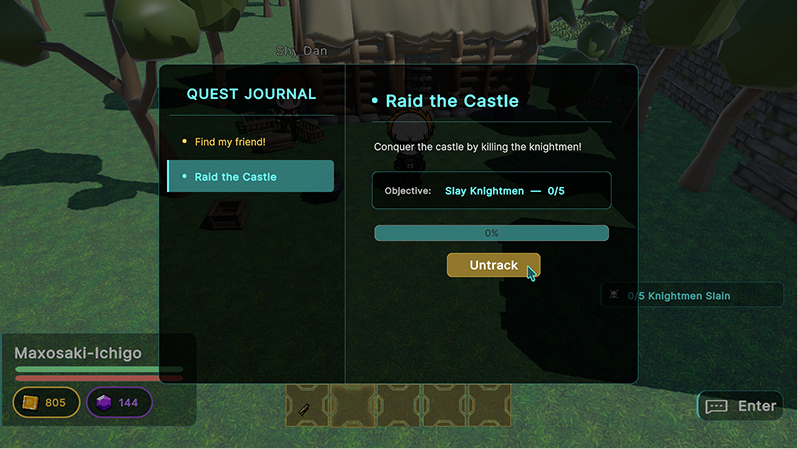
\includegraphics[width=0.85\textwidth]{img/08-implemented-solution/product/quest-journal.jpg}
    \caption{Captura de pantalla del diario de misiones.}    \label{fig:quest-journal}
\end{figure}
